\documentclass{article}
\usepackage{graphicx,psfrag,epsfig,epsf,latexsym,hhline,amsmath,amssymb,multirow}
\usepackage[usenames,dvipsnames]{pstricks}
\usepackage{pst-plot}
\usepackage{pstricks-add}
\usepackage{color}
\usepackage{stmaryrd}
\usepackage{makecell}

\interdisplaylinepenalty=2500
\usepackage{graphicx}
\usepackage{amsthm}
\usepackage{footnote}

\usepackage{blindtext}
\usepackage{etoolbox}

\usepackage{tikz}
\usepackage{pgfplots}
\usepgflibrary{shapes}
\usetikzlibrary{arrows,shapes,chains,matrix,positioning,scopes,patterns	}
\pgfplotsset{compat=newest}
\pgfplotsset{plot coordinates/math parser=false}

\begin{document}

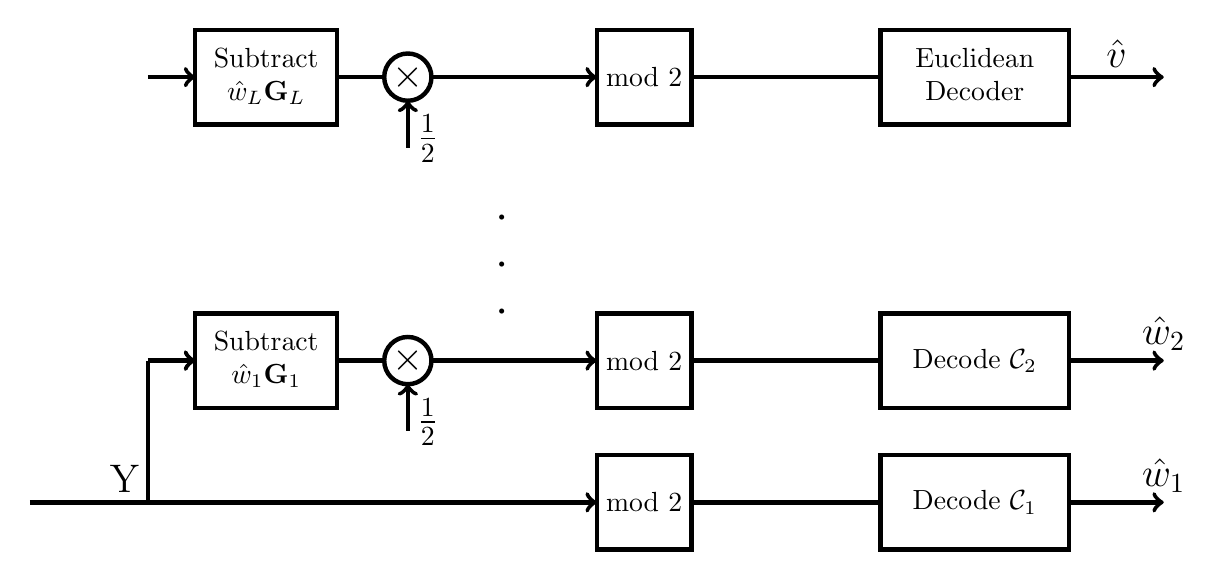
\begin{tikzpicture}[scale=0.6]

%Level 1 -mod2
\draw[->,ultra thick] (-10,1) -- (2,1);  \node [above, font=\Large] at (-8,1){Y} ;
\draw [ultra thick] (2,0) rectangle (4,2); \node [font=\normalsize] at (3,1){mod 2} ;

%Level 1- Decoder
\draw[ultra thick] (4,1) -- (8,1);
\draw [ultra thick] (8,0) rectangle (12,2);\node [font=\normalsize] at (10,1){Decode $\mathcal{C}_{1}$} ;
\draw[->,ultra thick] (12,1) -- (14,1);\node [above,font=\Large] at (14,1){$\hat{w}_{1}$};

%At Level 2 -  subtract
\draw[ultra thick] (-7.5,1) -- (-7.5,4); \draw[->,ultra thick] (-7.5,4) -- (-6.5,4);
\draw [ultra thick](-6.5,3) rectangle (-3.5,5); \node [font=\normalsize] at (-5,4){\makecell{Subtract\\ $\hat{w}_{1} \mathbf{G}_1$}} ;

%1/2 Multiplication block
\draw [ultra thick](-3.5,4) -- (-2.5,4);
\draw [ultra thick](-2,4) circle (0	.5); \node [font=\Large] at (-2,4){$\times$} ;
\draw[<-,ultra thick] (-2,3.5) -- (-2,2.5);
\node [right,font=\Large] at (-2,2.7){$\frac{1}{2}$} ;
\draw[->,ultra thick] (-1.5,4) -- (2,4);

%Level 2 Decoder
\draw [ultra thick] (2,3) rectangle (4,5); \node [font=\normalsize] at (3,4){mod 2} ;
\draw[ultra thick] (4,4) -- (8,4);
\draw [ultra thick] (8,3) rectangle (12,5);\node [font=\normalsize] at (10,4){Decode $\mathcal{C}_{2}$} ;
\draw[->,ultra thick] (12,4) -- (14,4);\node [above,font=\Large] at (14,4){$\hat{w}_{2}$};

%cdots
\node [font=\LARGE] at (0,5){$\cdot$} ;
\node [font=\LARGE] at (0,6){$\cdot$} ;
\node [font=\LARGE] at (0,7){$\cdot$} ;

%At Level L+1- subtract and halve it
 \draw[->,ultra thick] (-7.5,10) -- (-6.5,10);
\draw[->,ultra thick] (-7.5,4) -- (-6.5,4);
\draw [ultra thick](-6.5,9) rectangle (-3.5,11);  \node [font=\normalsize] at (-5,10){\makecell{Subtract\\ $\hat{w}_{L} \mathbf{G}_L$}} ;

\draw [ultra thick](-3.5,10) -- (-2.5,10);
\draw [ultra thick](-2,10) circle (0.5); \node [font=\Large] at (-2,10){$\times$} ;
\draw[<-,ultra thick] (-2,9.5) -- (-2,8.5);
\node [right,font=\Large] at (-2,8.7){$\frac{1}{2}$} ;
\draw[->,ultra thick] (-1.5,10) -- (2,10);

%Level L Decoder
\draw [ultra thick] (2,9) rectangle (4,11); \node [font=\normalsize] at (3,10){mod 2} ;
\draw[ultra thick] (4,10) -- (8,10);
\draw [ultra thick] (8,9) rectangle (12,11);\node [font=\normalsize] at (10,10){\makecell{Euclidean\\ Decoder}} ;
\draw[->,ultra thick] (12,10) -- (14,10);\node [above,font=\Large] at (13,10){$\hat{v}$};

 \end{tikzpicture}
\end{document} 